\subsection{Resolved Comparator Evidence}
\label{sec:resolved-3d-comparison}

\subsubsection{Available Resolved Data and Matching Limits}
\label{subsec:preliminary-cross-model-velocity-comparison}

This section reports final-time comparisons between the selected 1D
area--flow solution and two resolved stenotic-vessel datasets. The retained
datasets are the 23\% stenosis case from local dataset 77 and the 40\%
stenosis case from local dataset 60. Both are sampled at
$T=0.9995\,\mathrm{s}$; the recorded 1D--3D final-time offset is
$5.47\times10^{-14}\,\mathrm{s}$ in each case. This timestamp agreement is a
final-time alignment check, not a complete transient-history match.

The evidence below separates three resolved-comparator questions. First, the
reference-coordinate velocity comparison maps the 1D and 3D fields to common
section-mean observables. Second, the deformed-coordinate comparison applies the
available node-centered displacement field before forming plane cuts. Third,
the quasi-static membrane-FSI solve supplies a resolved wall-deformation
comparator based on the membrane relation used by Canic et al.\ for their wall
model \cite[Eq.~(35)]{CanicEtAl2024Extended1DStenosis}. The third item is a
Canic-style resolved comparator for this report, not a reproduction of the full
transient FSI calculation in that paper.

\begin{table}[!htb]
    \centering
    \scriptsize
    \caption{Resolved-data metadata used by the velocity and
    displacement-aware comparisons. Dataset identifiers are provenance labels;
    the case descriptions in the text use stenosis severity.}
    \label{tab:resolved-3d-metadata}
    \resizebox{\textwidth}{!}{%
    \begin{tabular}{@{}lrrrrllll@{}}
        \toprule
        \textbf{Case}
            & \textbf{Dataset}
            & \textbf{Nodes}
            & \textbf{Tetra.}
            & $\boldsymbol{t_{3D}}$ \textbf{(s)}
            & $\boldsymbol{|t_{3D}-T|}$ \textbf{(s)}
            & \textbf{Velocity}
            & \textbf{Pressure}
            & \textbf{Displacement} \\
        \midrule
        23\% stenosis & 77 & 22691 & 110420 & 0.9995 & $5.47\times10^{-14}$ & node-centered & node-centered & applied in deformed-coordinate cuts \\
        40\% stenosis & 60 & 21975 & 106547 & 0.9995 & $5.47\times10^{-14}$ & node-centered & node-centered & applied in deformed-coordinate cuts \\
        \bottomrule
    \end{tabular}%
    }
\end{table}

\begin{figure}[!htb]
    \centering
    \captionsetup{aboveskip=2pt,belowskip=2pt}
    \IfFileExists{report/assets/rendered/resolved-3d-flow-field.pdf}{%
        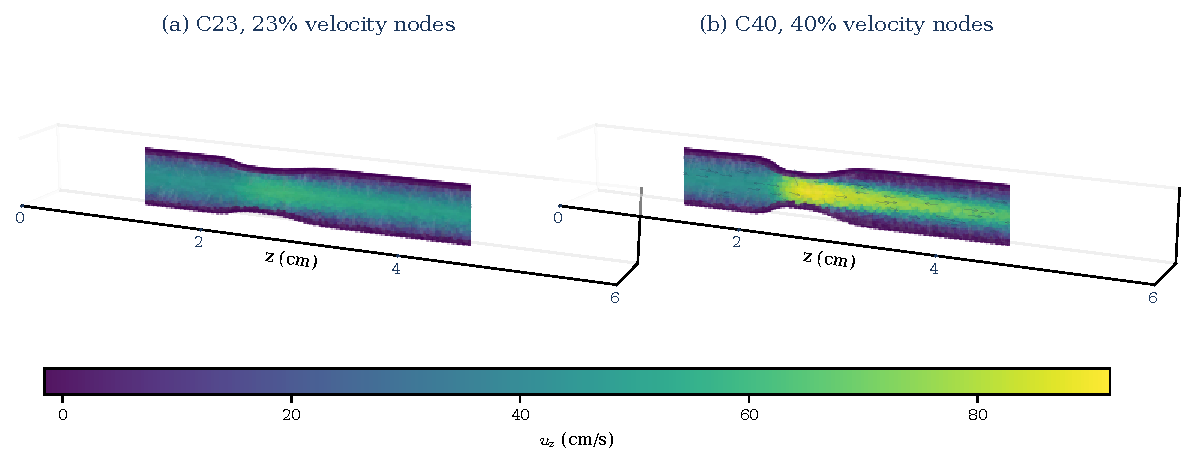
\includegraphics[width=\textwidth]{report/assets/rendered/resolved-3d-flow-field.pdf}
    }{%
        \fbox{\parbox{0.82\linewidth}{\centering Resolved velocity-field
        asset unavailable in this checkout.}}
    }
    \caption{Final-time resolved velocity samples used by the 23\% and 40\%
    stenosis comparisons. The panels show node-centered $u_z$ values; the
    quantitative comparison enters only after applying the declared
    cross-sectional observation operator.}
    \label{fig:resolved-3d-flow-field}
\end{figure}

\begin{table}[!htb]
    \centering
    \scriptsize
    \caption{Subcritical-boundary diagnostics for the same two 1D runs used in
    the resolved-velocity comparison. The characteristic-radicand values are in
    solver units of cm$^2$/s$^2$; the signs of $\lambda_-$ and $\lambda_+$
    support the boundary-regime gate in
    Assumption~\ref{ass:1d-subcritical-boundary-regime}.}
    \label{tab:t1-alpha-radicand-diagnostics}
    \resizebox{\textwidth}{!}{%
    \begin{tabular}{@{}lrrrrrrrr@{}}
        \toprule
        \textbf{Case}
            & $\boldsymbol{\min \alpha_{\mathrm{eff}}}$
            & $\boldsymbol{\max \alpha_{\mathrm{eff}}}$
            & $\boldsymbol{\min \chi^2}$
            & $\boldsymbol{\min\lambda_-}$
            & $\boldsymbol{\max\lambda_-}$
            & $\boldsymbol{\min\lambda_+}$
            & $\boldsymbol{\max\lambda_+}$
            & $\boldsymbol{\min\{\lambda_+,-\lambda_-\}}$ \\
        \midrule
        23\% stenosis & 1.33058 & 1.33333 & $8.15\times 10^5$ & -998.85 & -852.17 & 953.33 & 1058.76 & 852.17 \\
        40\% stenosis & 1.32500 & 1.33333 & $6.36\times 10^5$ & -999.08 & -713.79 & 880.69 & 1058.94 & 713.79 \\
        \bottomrule
    \end{tabular}
    }
\end{table}

\begin{table}[!htb]
    \centering
    \scriptsize
    \pgfplotstableread[col sep=space]{report/assets/data/stenosis-comparison/production-diagnostics-reference.dat}\TOneProductionDiagnostics
    \caption{Production diagnostics from the 23\% and 40\% severity 1D
    comparison runs completed at $T=0.9995$ s. These rows summarize timestep,
    CFL, positivity, area, and finite-volume bookkeeping for the 1D runs used
    in the resolved-comparator evidence.}
    \label{tab:t1-production-diagnostics}
    \resizebox{\textwidth}{!}{%
    \pgfplotstabletypeset[
        columns={
            case,
            target_time,
            completed_time,
            cross_model_time_offset,
            dt_min,
            dt_max,
            cfl_max,
            min_Aphys,
            volume_defect,
            positivity_count,
            area_flux_balance,
            rhs_area_max,
            rhs_flow_max
        },
        every head row/.style={before row=\toprule, after row=\midrule},
        every last row/.style={after row=\bottomrule},
        columns/case/.style={string type,column type=l,column name=\textbf{Stenosis}},
        columns/target_time/.style={fixed,precision=4,column name=$\boldsymbol{T_{\mathrm{target}}}$},
        columns/completed_time/.style={fixed,precision=4,column name=$\boldsymbol{T_{\mathrm{done}}}$},
        columns/cross_model_time_offset/.style={sci,precision=2,column name=$\boldsymbol{|\Delta t_{\mathrm{1D--3D}}|}$},
        columns/dt_min/.style={sci,precision=2,column name=$\boldsymbol{\Delta t_{\min}}$},
        columns/dt_max/.style={sci,precision=2,column name=$\boldsymbol{\Delta t_{\max}}$},
        columns/cfl_max/.style={fixed,precision=2,column name=\textbf{CFL$_{\max}$}},
        columns/min_Aphys/.style={fixed,precision=5,column name=$\boldsymbol{\min \pi a}$},
        columns/volume_defect/.style={sci,precision=2,column name=$\boldsymbol{\Delta\!\int a\,dz}$},
        columns/positivity_count/.style={int detect,column name=\textbf{pos. count}},
        columns/area_flux_balance/.style={sci,precision=2,column name=\textbf{area-flux balance}},
        columns/rhs_area_max/.style={sci,precision=2,column name=$\boldsymbol{\max|\dot a|}$},
        columns/rhs_flow_max/.style={fixed,precision=5,column name=$\boldsymbol{\max|\dot q|}$}
    ]\TOneProductionDiagnostics
    }
\end{table}

\FloatBarrier

\subsubsection{Observation Operator and Deformed Coordinates}
\label{subsec:cross-sectional-sampling-protocol-results}

The comparison uses the declared \texttt{CrossSectionQuadratureOperator}. For a
target plane $S_j=\Omega_{\mathrm{3D}}\cap\{z=z_j\}$, the operator intersects
the tetrahedral mesh with the plane, triangulates the cut polygon, and computes
\begin{flalign*}
    \quad
    A_{3D,j}
    =
    \sum_{\Delta\in\mathcal Q_j}|\Delta|,
    \qquad
    Q_{3D,j}
    =
    \sum_{\Delta\in\mathcal Q_j}|\Delta|\,\bar u_{z,\Delta},
    \qquad
    \bar u_{3D,j}
    =
    Q_{3D,j}/A_{3D,j}. &&
\end{flalign*}
The 1D quantities use the solver-to-physical map
$Q_{1D,j}=\pi q(z_j,t)$ and $\bar u_{1D,j}=q(z_j,t)/a(z_j,t)$. In
deformed-coordinate mode the plane cut is formed after replacing each mesh
coordinate $x$ by $x+d(x)$, where $d$ is the node-centered resolved
displacement field.

The stenosis throat is the minimizer $z^\star=\argmin_z R_0(z)$ of the smooth
reference-radius profile in Eq.~\ref{eq:1d-stenosis-profile}. For the comparison
geometry this gives $z^\star\approx2.451\,\mathrm{cm}$, with
$R_{\min}=0.1386\,\mathrm{cm}$ for the 23\% stenosis case and
$R_{\min}=0.1080\,\mathrm{cm}$ for the 40\% stenosis case.

\begin{table}[!htb]
    \centering
    \scriptsize
    \caption{Cut-area check against the static reference
    $A_{\mathrm{ref}}(z)=\pi R_0(z)^2$ for both coordinate choices.
    Discrepancies are percentages over the 200 valid section targets.}
    \label{tab:t1-area-check}
    \begin{tabular}{@{}llrrrr@{}}
        \toprule
        \textbf{Case}
            & \textbf{Coordinates}
            & $\boldsymbol{\min \epsilon_A}$
            & $\boldsymbol{\mathrm{median}\ \epsilon_A}$
            & $\boldsymbol{\mathrm{mean}\ \epsilon_A}$
            & $\boldsymbol{\max \epsilon_A}$ \\
        \midrule
        23\% stenosis & reference & 0.045 & 0.281 & 0.389 & 2.94 \\
        23\% stenosis & deformed & 0.001 & 0.254 & 0.336 & 3.03 \\
        40\% stenosis & reference & 0.005 & 0.291 & 0.397 & 4.46 \\
        40\% stenosis & deformed & 0.003 & 0.286 & 0.417 & 4.60 \\
        \bottomrule
    \end{tabular}
\end{table}

\subsubsection{Reference-Coordinate Velocity Comparison}
\label{subsec:section-mean-velocity-discrepancies}

The reference-coordinate comparison is retained as the baseline final-time
velocity comparison. The section means are
$\langle Q_{1D}\rangle=2.288\,\mathrm{cm}^3/\mathrm{s}$ and
$\langle Q_{3D}\rangle=2.241\,\mathrm{cm}^3/\mathrm{s}$ for the 23\% stenosis
case, and $\langle Q_{1D}\rangle=2.287\,\mathrm{cm}^3/\mathrm{s}$ and
$\langle Q_{3D}\rangle=2.219\,\mathrm{cm}^3/\mathrm{s}$ for the 40\% stenosis
case.

\begin{figure}[!htb]
    \centering
    \captionsetup{aboveskip=2pt,belowskip=2pt}
    \figtikz{axial-flow-comparison}
    \caption{Axial physical-flow comparison after applying the
    reference-coordinate plane-quadrature observation operator. Dashed curves
    are $Q_{1D}(z)=\pi q(z)$ and solid curves are $Q_{3D}(z)$ from the resolved
    velocity fields; the figure compares observed section flow, not native
    resolved velocity fields or pressure-ratio output.}
    \label{fig:t1-axial-flow-comparison}
\end{figure}

The algebraic split used for flow/area bookkeeping is
\begin{flalign*}
    \quad
    \frac{Q_{1D}}{A_{1D}}-\frac{Q_{3D}}{A_{3D}}
    =
    \frac{Q_{1D}-Q_{3D}}{A_{1D}}
    +
    Q_{3D}\left(\frac{1}{A_{1D}}-\frac{1}{A_{3D}}\right),
    \qquad A_{1D}=\pi a. &&
\end{flalign*}
This decomposition is bookkeeping for the sampled sections, not causal
attribution.

\begin{table}[!htb]
    \centering
    \scriptsize
    \caption{Section-wise decomposition of the reference-coordinate
    mean-velocity discrepancy into physical-flow and area-denominator
    contributions. Values are in cm/s. This bookkeeping split is tied to the
    declared section observation operator and is not a causal error
    attribution.}
    \label{tab:t1-flow-area-decomposition}
    \resizebox{\textwidth}{!}{%
    \begin{tabular}{@{}lrrrrl@{}}
        \toprule
        \textbf{Case}
            & $\boldsymbol{\langle |(Q_{1D}-Q_{3D})/A_{1D}|\rangle}$
            & $\boldsymbol{\langle |Q_{3D}(A_{1D}^{-1}-A_{3D}^{-1})|\rangle}$
            & $\boldsymbol{z_{\max |d_u|}}$
            & $\boldsymbol{|d_u|_{\max}}$
            & \textbf{Larger bookkeeping term at max} \\
        \midrule
        23\% stenosis & 0.529 & 0.112 & 2.291 & 2.35 & Flow term \\
        40\% stenosis & 1.012 & 0.133 & 2.261 & 9.92 & Flow term \\
        \bottomrule
    \end{tabular}%
    }
\end{table}

\begin{table}[!htb]
    \centering
    \scriptsize
    \caption{Reference-coordinate section-mean velocity discrepancy summary at
    the matched final-time sample after applying the common section observation
    map. Values are in cm/s except for the axial location column in cm; the
    table reports diagnostic cross-model discrepancy, not clinical validation.}
    \label{tab:t1-3d-comparison-summary}
    \resizebox{\textwidth}{!}{%
    \begin{tabular}{@{}lrrrrrrrrr@{}}
        \toprule
        \textbf{Case}
            & \textbf{Sections}
            & $\boldsymbol{\langle\bar u_{1D}\rangle}$
            & $\boldsymbol{\langle\bar u_{3D}\rangle}$
            & $\boldsymbol{\overline d_u}$
            & $\boldsymbol{D_{u,1}}$
            & $\boldsymbol{D_{u,2}}$
            & \textbf{rel.} $\boldsymbol{D_{u,2}}$
            & $\boldsymbol{\max |d_u|}$
            & $\boldsymbol{z_{\max |d_u|}}$ \\
        \midrule
        23\% stenosis & 200 & 24.11 & 23.63 & 0.480 & 0.505 & 0.664 & 0.0277 & 2.35 & 2.291 \\
        40\% stenosis & 200 & 26.43 & 25.52 & 0.909 & 0.966 & 1.87 & 0.0688 & 9.92 & 2.261 \\
        \bottomrule
    \end{tabular}
    }
\end{table}

\begin{figure}[!htb]
    \centering
    \captionsetup{aboveskip=2pt,belowskip=2pt}
    \figtikz{section-mean-comparison}
    \caption{Area-mean axial velocity comparison at $t=0.9995$ s under the
    reference-coordinate section observation map. Solid curves are tetrahedral
    cross-section quadrature means from the resolved 3D velocity field; dashed
    curves are interpolated 1D means
    $\bar u=q/a=Q_{\mathrm{phys}}/A_{\mathrm{phys}}$.}
    \label{fig:t1-section-mean-comparison}
\end{figure}

\begin{table}[!htb]
    \centering
    \scriptsize
    \caption{Normalized scale comparison between the production-grid
    geometry-rest limitation and final-time 1D--3D velocity-discrepancy
    measures. These ratios place the diagnostic comparison on a common scale;
    they do not convert the comparison into an accepted-reference validation
    result.}
    \label{tab:t1-normalized-scale-comparison}
    \begin{tabular}{@{}lrrrr@{}}
        \toprule
        \textbf{Case}
            & \textbf{rest }$\boldsymbol{\max |q|}$\textbf{/prod. }$\boldsymbol{q}$
            & $\boldsymbol{D_{Q,1}/\langle Q_{1D}\rangle}$
            & $\boldsymbol{D_{u,1}}$ \textbf{(cm/s)}
            & \textbf{rel. }$\boldsymbol{D_{u,2}}$ \\
        \midrule
        23\% stenosis & 5.27\% & 2.11\% & 0.505 & 2.77\% \\
        40\% stenosis & 8.71\% & 3.10\% & 0.966 & 6.88\% \\
        \bottomrule
    \end{tabular}
\end{table}

\begin{table}[!htb]
    \centering
    \scriptsize
    \caption{Optional production-grid sensitivity for the reference-coordinate
    resolved-velocity observation map. Flow discrepancies are in cm$^3$/s and
    velocity discrepancies are in cm/s; the rows test numerical sensitivity of
    the comparison output, not patient-specific interpretation.}
    \label{tab:t1-grid-sensitivity-summary}
    \resizebox{\textwidth}{!}{%
    \begin{tabular}{llrrrrrrr}
\toprule
Case & $N$ & $D_{Q,1}$ & $D_{Q,2}$ & $D_{u,1}$ & $D_{u,2}$ & rel. $D_{u,2}$ & max $|d_u|$ & adj. $D_{u,2}$ \\
\midrule
23\% stenosis & 200 & 0.05965 & 0.07358 & 0.6182 & 0.8996 & 0.03757 & 4.533 & -- \\
23\% stenosis & 400 & 0.04821 & 0.05085 & 0.5048 & 0.6636 & 0.02771 & 2.349 & 0.678 \\
23\% stenosis & 800 & 0.04874 & 0.05322 & 0.5049 & 0.7063 & 0.0295 & 2.94 & 0.1785 \\
40\% stenosis & 200 & 0.08395 & 0.1132 & 1.082 & 1.894 & 0.06975 & 7.93 & -- \\
40\% stenosis & 400 & 0.07087 & 0.08927 & 0.966 & 1.868 & 0.06881 & 9.923 & 1.328 \\
40\% stenosis & 800 & 0.07108 & 0.09539 & 0.9843 & 2.019 & 0.07435 & 11.57 & 0.3499 \\
\bottomrule
\end{tabular}
%
    }
\end{table}

\begin{table}[!htb]
    \centering
    \scriptsize
    \caption{Five largest section-wise velocity discrepancies in the
    reference-coordinate comparison. Velocities and velocity discrepancies are
    in cm/s; physical flows and flow discrepancies are in cm$^3$/s. The ranking
    identifies where the declared observation map differs most strongly between
    tiers.}
    \label{tab:t1-largest-section-discrepancies}
    \begin{tabular}{@{}rlrrrrrrrr@{}}
        \toprule
        \textbf{Rank}
            & \textbf{Case}
            & $\boldsymbol{z}$ \textbf{(cm)}
            & $\boldsymbol{\bar u_{1D}}$
            & $\boldsymbol{\bar u_{3D}}$
            & $\boldsymbol{|d_u|}$
            & $\boldsymbol{Q_{1D}}$
            & $\boldsymbol{Q_{3D}}$
            & $\boldsymbol{|d_Q|}$
            & \textbf{Tri.} \\
        \midrule
        1 & 40\% stenosis & 2.261 & 52.58 & 42.66 & 9.92 & 2.201 & 1.862 & 0.339 & 759 \\
        2 & 40\% stenosis & 2.291 & 56.94 & 48.20 & 8.74 & 2.230 & 1.903 & 0.327 & 749 \\
        3 & 40\% stenosis & 2.352 & 61.43 & 53.22 & 8.21 & 2.270 & 1.980 & 0.290 & 743 \\
        4 & 40\% stenosis & 2.322 & 59.81 & 52.09 & 7.72 & 2.253 & 1.970 & 0.283 & 771 \\
        5 & 40\% stenosis & 2.231 & 46.95 & 39.94 & 7.01 & 2.174 & 1.918 & 0.256 & 833 \\
        \bottomrule
    \end{tabular}
\end{table}

\subsubsection{Deformed-Coordinate Comparison}
\label{subsec:deformed-coordinate-comparison}

The deformed-coordinate comparison repeats the same section operator after
moving each resolved node by its displacement value. Table~\ref{tab:t1-coordinate-mode-comparison}
shows that applying displacement changes the final-time discrepancy measures
only modestly for these two datasets. This is still not a full wall-motion
match: the available comparison record contains the final displacement field, not the
resolved wall history or boundary histories.

\begin{table}[!htb]
    \centering
    \scriptsize
    \caption{Reference-coordinate versus deformed-coordinate discrepancy
    measures for the same section observation map. $D_{u,1}$ and $D_{u,2}$ are
    the mean absolute and RMS section-mean velocity discrepancies in cm/s;
    $D_{Q,1}$ is the mean absolute physical-flow discrepancy in cm$^3$/s.}
    \label{tab:t1-coordinate-mode-comparison}
    \begin{tabular}{@{}llrrrr@{}}
\toprule
Case & Coordinates & $D_{u,1}$ & $D_{u,2}$ & $\max |d_u|$ & $D_{Q,1}$ \\
\midrule
C23 (22.56\%) & reference & 0.6040 & 1.070 & 11.400 & 0.06259 \\
C23 (22.56\%) & deformed & 0.6111 & 1.073 & 11.400 & 0.06184 \\
40\% stenosis & reference & 1.1318 & 2.292 & 12.291 & 0.08514 \\
40\% stenosis & deformed & 1.1410 & 2.294 & 12.304 & 0.08420 \\
\bottomrule
\end{tabular}

\end{table}

\begin{figure}[!htb]
    \centering
    \captionsetup{aboveskip=2pt,belowskip=2pt}
    \figtikz{coordinate-mode-discrepancy}
    \caption{Effect of the displacement-aware observation map on the
    section-wise velocity discrepancy. Solid curves use reference mesh
    coordinates, while dashed curves form the same plane cuts after the nodal
    map $x\mapsto x+d(x)$; the figure changes the coordinate mode, not the 1D
    model or the resolved velocity field.}
    \label{fig:t1-coordinate-mode-discrepancy}
\end{figure}

\subsubsection{Quasi-static Membrane-FSI Comparator}
\label{subsec:membrane-fsi-comparator}

The resolved wall comparator solves a quasi-static fixed point between the
Stokes lumen solve and the radial membrane update. In the notation of
Appendix~\ref{app:num-membrane-fsi-validation}, the wall equation is the
inertia-free form
\begin{flalign*}
    \quad
    C_0\eta_r(z)=f_r(z),
    \qquad
    \eta_r(0)=\eta_r(L)=0,
    \qquad
    C_0=\frac{Eh}{(1-\sigma^2)(R_0^*)^2}. &&
\end{flalign*}
This is the Canic-style membrane relation used for the resolved comparator
\cite[Eq.~(35)]{CanicEtAl2024Extended1DStenosis}. It is separate from the
selected 1D pressure--area closure used in the reduced model. The retained
comparator is a quasi-static radial membrane update coupled to repeated Stokes
solves; it informs wall-motion scale, not full transient moving-boundary FSI
validation.

\begin{table}[!htb]
    \centering
    \scriptsize
    \caption{Quasi-static membrane-FSI fixed-point results on the retained
    finer mesh. The reported displacement is the radial wall displacement
    $\eta_r$; the minimum radius is the deformed lumen radius
    $R_0+\eta_r$. This comparator informs wall-motion scale only and does not
    supply a transient FSI validation target.}
    \label{tab:t1-membrane-fsi-summary}
    \begin{tabular}{@{}lrrrrrr@{}}
\toprule
Case & Mesh & Iter. & Residual (cm) & $\max\eta$ (cm) & $\min R$ (cm) & $\langle Q\rangle$ (cm$^3$/s) \\
\midrule
C23 (22.56\%) & $16\times4\times16$ & 9 & 5.972e-8 & 3.052e-5 & 0.1402 & 0.5472 \\
40\% stenosis & $16\times4\times16$ & 9 & 6.051e-8 & 3.092e-5 & 0.1108 & 0.416 \\
\bottomrule
\end{tabular}

\end{table}

\begin{figure}[!htb]
    \centering
    \captionsetup{aboveskip=2pt,belowskip=2pt}
    \resizebox{0.98\textwidth}{!}{\figtikz{membrane-fsi-wall-profile}}
    \caption{Quasi-static wall deformation from the membrane-FSI comparator.
    The upper panel shows the radial displacement $\eta_r(z)$ solving the
    fixed-end membrane equation; the lower panel shows the resulting deformed
    radius $R_0(z)+\eta_r(z)$ alongside the reference radius.}
    \label{fig:t1-membrane-fsi-wall-profile}
\end{figure}

\begin{figure}[!htb]
    \centering
    \captionsetup{aboveskip=2pt,belowskip=2pt}
    \resizebox{0.98\textwidth}{!}{\figtikz{membrane-fsi-fixed-point-history}}
    \caption{Fixed-point convergence for the quasi-static membrane-FSI
    comparator. The residual is the maximum radial-radius update between
    successive coupled wall solves, reported in centimeters; it checks the
    comparator solve, not the 1D--3D velocity observation error.}
    \label{fig:t1-membrane-fsi-fixed-point-history}
\end{figure}

\subsubsection{Radial-Profile Audit}
\label{subsec:reconstructed-radial-profile-results}

The radial-profile reducer was rerun for slices
$z=1.951$, $2.451$, and $2.951\,\mathrm{cm}$ in both reference and deformed
coordinate modes. Its summary-discrepancy recomputation matched the generated
radial summaries, but the area-closure gate failed because those slices are not
members of the retained 200-section axial target set. The radial-profile plot is
therefore not promoted into the main evidence.

\begin{table}[!htb]
    \centering
    \scriptsize
    \caption{Radial-profile promotion check. The zero summary delta confirms
    that the raw radial rows reproduce the generated radial-summary statistic;
    the area-closure gate remains failed, so no radial figure or radial-bin
    localization claim is retained.}
    \label{tab:t1-radial-profile-audit}
    \begin{tabular}{@{}llrrrl@{}}
\toprule
Case & Coordinates & Slices & Bins & Summary delta & Audit result \\
\midrule
C23 (22.56\%) & reference & 3 & 20 & 0.0 & not_evaluated: matching section row unavailable at radial z-slice; section area unavailable; section flow unavailable \\
C23 (22.56\%) & deformed & 3 & 20 & 0.0 & not_evaluated: matching section row unavailable at radial z-slice; section area unavailable; section flow unavailable \\
40\% stenosis & reference & 3 & 20 & 0.0 & not_evaluated: matching section row unavailable at radial z-slice; section area unavailable; section flow unavailable \\
40\% stenosis & deformed & 3 & 20 & 0.0 & not_evaluated: matching section row unavailable at radial z-slice; section area unavailable; section flow unavailable \\
\bottomrule
\end{tabular}

\end{table}

\subsubsection{Interpretation Limits}
\label{subsec:spatial-localization-discrepancies}

This chapter reports a controlled diagnostic cross-model comparison against
declared resolved comparators: a reference-coordinate velocity comparison, a
displacement-aware observation comparison, and a quasi-static membrane-wall
comparator. The evidence supports the implemented observation and comparison
workflow and localizes final-time velocity discrepancies under the stated
operators. It does not provide externally validated clinical prediction
evidence, pressure-ratio evidence, or equivalence to a full transient FSI
computation with matched boundary and wall-history data.
